\section{Preiskovanje}

\subsection{Neinformirani preiskovalni algoritmi}

\subsubsection{Iskanje v sirino}

\subsubsection{iskanje v globino}

Izboljsave:
\begin{itemize}
    \item \textbf{Iskanje s sestopanjem}
    \item \textbf{depth-limited-search} (vnapej definiramo globino l (dolocimo preko domenskega znanja))
\end{itemize}

\subsubsection{iterativno poglabljanje}
problem gobinsko omejenega iskanja -> nastavitev meje l
Mejo l postopoma povecujemo za 1, dokler ne najdemo resitve.
% itemize without spacing
\begin{itemize}[noitemsep,topsep=0pt]
    \item \textbf{popolnost}: Da
    \item \textbf{optimalnost}: Da
    \item \textbf{casovna zahtevnost} $O(b^d)$
    \item \textbf{prostorska zahtevnost} $O(bd)$
\end{itemize}
Boljse od iskanja v globino/sirino

\subsubsection{dvosmerno iskanje}
Ideja: pognati vzporedni iskanji od zacetka do cilja in od cilja do zacetka.\\
Motivacija: \\ 

\textbf{Implemenatcija dvosmernega iskanja}

\begin{itemize}[noitemsep,topsep=0pt,leftmargin=*]
    \item ciljno vozlisce mora biti znano
    \item originalni problemski prostor preslikamo v dvosmerni prosto stanj
    E1, E2 dosegljiv iz E in S1,S2,S3 dosegljiv iz S
    (S,E) -> {(S1, E1), (S1,E2), (S2, E1), (S2, E2)...}
    Vozlisce (Si, Ei) je v dvosmernem prostur ciljo vozlisce ce velja E=S (soda dolzina na isto mesto pridemo iz obeh strani) ali S->E (liha pot sosednja)
\end{itemize}


\subsection{Informirani preiskovalni algoritmi}

\subsubsection{Hevristicno preiskovanje - Hevristika}
ideja: preiskovanje usmerjamo z dodatnim znanjem \textbf{hevristika} je ocenitvena funkcija za obetavnost vozlisca\\
- \green{optimisticna/dopustna}: $\forall n: \bm{h(n) \leq h^*(n)}$ ($h^*$ je optimalna ocena)\\
- \green{optimalna}: $h(n) = h^*(n)$\\
- \green{pesimisticna}: $h(n) \geq h^*(n)$

\subsubsection{A*}
A* is informed version of \textbf{dijkstra} (uses heuristics and pq), ce h(dopustna)=\textbf{popolna in optimalna}\\
\textbf{Casovna zahtevnost} odvisna od hevristike: $E = (h^* - h)/h^*$, $O(b^{E \cdot d})$, b-stopnja vejanja, d-globina optimalne resitve\\ 
\textbf{Prostorska zahtevnost} \textbf{problem} (hrani vsa vozlisca v spominu)\\
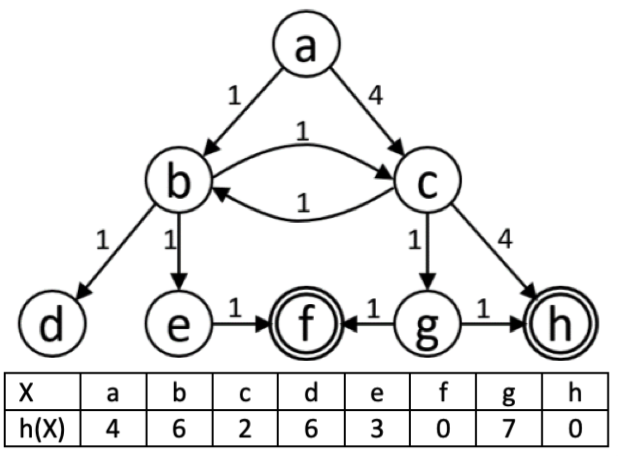
\includegraphics[width=3cm]{./images/graf-a.png}\\
$f(n)=g(n)+h(n)$, g(n) cena do vozlisca, h(n) hevristika\\
Razvijamo dokler ne pridemo do ciljnega vozlisca\\
\begin{tabular}{c|c|c}
    Razvijano & Generirana & Priority Queue\\
    \hline
    / & a(4) & [] \\
    a & b(7) c(6) & $\left[ c(6), b(7)\right]$\\
    c & b'(11) g(12) h(8) & [b(7),h(8),b'(11),g(12)]\\
    b & c'(4) d(8) e(5) & [c'(4),e(5),h(8),d(8),b'(11),g(12)]\\
    \dots & \dots & \dots\\
    \magenta{f} & &
\end{tabular}

\subsubsection{IDA* (Iterative deepening A*)}
f(n) = g(n) + h(n), g(n)=cena poti do n\\
\begin{tabular}{c|c|c|c}
    Meja & Razvijano & Generirana & DFS (list)\\
    \hline
    0 & / & s(7) & /\\
    \hline
    7 & / & s(7) & s \\
      & s & a(8) b(7) c(7) & b, c\\
      & b & f(6) h(5) & f h c\\
      & f & g(7) h(9) i(11) & g h c\\
      & \underline{g} &  & 
\end{tabular}



\subsubsection{Kakovost hevristicnih funkcij}

Kakovost h ocenimo z \textbf{stevilom generiranih vozlisc} ter \textbf{efektivnim faktorjem vejanja} (N vozlisc je algoritem generiral da je na globini d nasel resitev)\\
Hocemo imeti dopustne hevristike s \textbf{cim visjimi vrednostmi} in \textbf{sprejelmjivo ceno} (casom izracuna)\\
Ce $h_2(n) \geq h_1(n), \forall n$ potem $h_2$ \textbf{dominira} $h_1$\\


\subsection{Lokalno preiskovalni algoritmi}

\subsubsection{Plezanje na hrib}
Ne pomnemo poti do cilja, ampak samo trenutno stanje\\
Koristni v primerih:\\
- ce nas zanima samo kakovost resitve (in ne pot do cilja)\\
- resevanje optimizacijskih problemov (kjer je podana \textbf{kriterijska funkcija} za oceno kakovosti resitve)\\

Prednosti:\\
- majhna poraba prostora\\

\textbf{Primer 4 kraljice na sahovnici}
- kriterijska funkcija: maksimiziramo - (minus) stevilo kraljic, ki se medsebojno napadajo

Tezave:
\begin{itemize}[noitemsep,topsep=0pt,leftmargin=*]
    \item lokalni maksimumi
    \item "rame, plaote" (kriterijska funkcija konstantna vrednost)
    \item grebeni (za plezanje navzgor je potreben sestop po pobocju grebena)
\end{itemize}

Resevanje iz lokalnih maksimumov:
\begin{itemize}[noitemsep,topsep=0pt,leftmargin=*]
    \item \textbf{koraki vstran}: ce ima naslednje stanje isto vrednost kriterijske funkcie, dovolimo premik v to stanje
    \item \textbf{stohasticno} plezanje na hrib: iz mnozice boljsih stanj, verjetnostno izberemo naslednje stanje (pri cemer upostevamo da imajo boljsa stanja vecjo verjetnost izbora)
    \item \textbf{nakljucni ponovni zagon}: veckrat pozeni plezanje na hrib iz nakljucnih stanj dokler ne najdes resitve
\end{itemize}

\subsubsection{Simulirano ohlajanje}
algoritem ki izvira iz metalurgije (ko je jeklo tekoce, so molekule v njem bolj gibljive; ko se ohlaja se strjuje in molekuele se umirjajo)
Analogija:\\
- generiramo nakljucne sosede trenutnega stanja\\
- ce najdemo \textbf{boljse stanje ga izberemo}\\
- ce najdemo \textbf{slabse stanje, ga izberemo z doloceno verjetnostjo}\\
- verjetnost izbire neoptimalnega stanja s casom pada (nizanje temperature)

\subsubsection{Lokalno iskanje v snopu}
Algoritem:\\
- v spominu hrani k aktualnih stanj namesto enega\\
- izberi k optimalnih stanj od sosedov aktualnih stanj\\
- ponavaljaj do ustavitnega pogoja 

\subsection{preiskovanje grafov AND/OR, nedeterministicno okolje}
Pomagajo resevati probleme z \textbf{dekompozicijo na manjse probleme}
Uporabnost:
\begin{itemize}[noitemsep,topsep=0pt,leftmargin=*]
    \item princip deli in vladaj
    \item iskanje v nedeterministicnih okoljih 
    \item igre med dvema nasprotnikoma s popolno informacijo (sah, dama)
    \item ekspertno resevanje problem
\end{itemize}
Primer graf dekompozicja v dva manjsa problema skozi g in f\\
\textbf{Resitveno drevo} je resitev AND/OR grafov\\
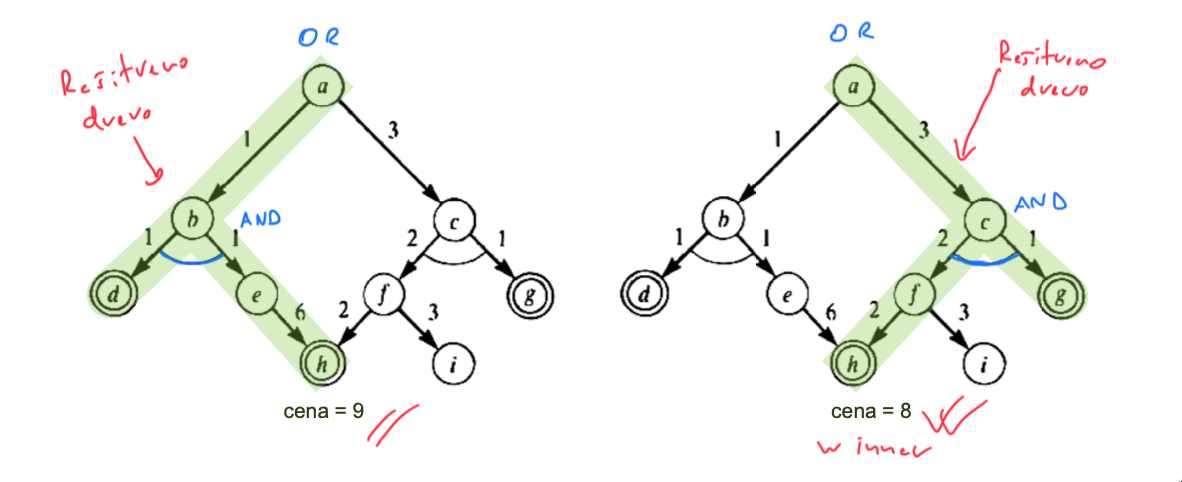
\includegraphics[width=6cm]{./images/resitveno-drevo.png}
\subsubsection{AO*}
\begin{itemize}[noitemsep,topsep=0pt,leftmargin=*]
    \item posplositev A* na grafe AND/OR
    \item \textbf{popoln in optimalen} $\Leftrightarrow$ h(n) ne precenjuje dejanske cene do cilja
\end{itemize}
$F(N) \dots$ ocena za usmerjanje preiskovanja\\ 
$H(N) \dots$ dinamicna hevristicna ocena\\
Postopek:
\begin{enumerate}[noitemsep,topsep=0pt,leftmargin=*]
    \item Razvij najcenejse vozlisce
    \begin{itemize}[noitemsep,topsep=0pt,leftmargin=*]
        \item ce list in koncno (oznaci), preveri 3. korak, nadaljuj v 1.
        \item ce list in ni koncno (oznaci) vrednost vozlisca = $\infty$
    \end{itemize}
    \item Posodobi vse predhodnike
    \begin{itemize}[noitemsep,topsep=0pt,leftmargin=*]
        \item v AND starsih, cena starsa = $\sum$ sinov + povezava v
        \item v OR starsih, cena starsa = min(sinovi) + povezava v
    \end{itemize}
    \item Koncaj ko obstaja pot od zacetnega vozlisca, po kateri v AND vozliscih po vseh sinovih prides do cilja, v OR vozliscih v vsaj enem
\end{enumerate}

\subsubsection{Preiskovanje v nedeterministicnem okolju:}
\textbf{Nedeterministican akcija} - ista akcija lahko obrodi razlicna ciljna stanja\\
Do resitve ni vec \textbf{poti} temvec \textbf{drevesa} (uporbljamo AND/OR grafe)\\
Vozsilca OR \textbf{mozne akcije}, vozlisca AND \textbf{vejanja v mozna stanja}, ki so rezultat nedeterministicnih akcij

\subsection{Preiskovanje brez informacij o stanju}
Okolja smo razdelili na \textbf{transparent} (agent lahko zazna popolno informacija) in \textbf{netransparentna} (brez informacije o stanju)\\
Kej ce imamo opravka z netraspranetim okoljem?\\
- izvajamo preiskovanje prostora \textbf{verjetnih} stanj in ne prostora \textbf{dejanskih} stanj\\
- izvajamo s postokopom omejevanja moznozsti kandidatnih stanj\

\subsection{Igranje iger}

\subsubsection{Predstavitev problema}

\subsubsection{algoritem MINIMAX}
- m globina
- b 

\subsubsection{Rezanje alfa-beta}
